\chapter{Problem and proposed solution} \label{chap:approach} \minitoc

\section{Scope}
The focus of this Thesis is the development of a lightweight real-time data monitoring system working in the presence of high volumes of high velocity, high variety, highly skewed and seasonal data. The resultant system should detect and report data pattern shifts in an unsupervised fashion. 

Essentially, the system will summarize incoming data with sliding window aggregations and probabilistic data structures in a sliding window fashion and compare current feature values with an initial given static configuration. Any big enough deviations between these two states should be reported as a data pattern shift.

Furthermore, the resulting system shall strive to achieve high precision and recall ratios as well as low latencies with a low memory footprint.


\section{Research Questions}
With this Thesis, we intend to build a system that monitors real-time data streams in a lightweight fashion. As such, in the end, to determine if the system is successful in doing so or not, the following research questions must be answered:

\begin{enumerate}[start=1, label={\textbf{RQ\arabic*:}}]
    \item Can the system accurately detect data pattern shifts --- \textit{i.e.} does it have \textbf{high precision ratio}?
    
    \item Can the system detect most of the data pattern shifts --- \textit{i.e.} does it have \textbf{high recall ratio}?
    
    \item Can the system detect data pattern shifts in real-time --- \textit{i.e.} does it work under extremely \textbf{low latencies}?
    
    \item Can the system detect data pattern shifts in a lightweight fashion --- \textit{i.e.} does it have a \textbf{low memory footprint}?

\end{enumerate}

\section{Experimental Methodology}

In order to validate or reject our proposed hypothesis, a set of tests will be carried out to determine the system's usefulness. The data sets used will belong to the financial fraud space. The output of the system will be compared to the results of an existing batch analysis tool, for the same data sets, both provided by Feedzai.

To test the stream monitoring system we will need a streaming engine. As such, either a custom-built streaming engine or an existing one --- \textit{e.g.} like Apache Flink \cite{Rabl-Apache-Flink} --- will be used. 

In brief, it is desired that our in real-time system monitoring report is as close to the batch analysis in terms of accuracy as possible.


\section{Planning}
To accomplish the proposed experiments, the following steps are required:

\begin{enumerate}[start=1, label={\textbf{T\arabic*:}}]
    \item \textbf{Research more state of the art aggregations} - search for more memory efficient sliding window aggregations to use in the final system.
    
    \item \textbf{Data set and batch results analysis} - explore chosen data sets and the resulting batch analysis made on them.
    
    \item \textbf{Stream Processing Engine (SPE) setup} - setup the stream processing engine chosen --- \textit{e.g.} Apache Flink \cite{Rabl-Apache-Flink} --- or build a custom very basic one.
    
    \item \textbf{Implementation of chosen algorithms} - implement the selected algorithms in an efficient programming language --- \textit{e.g.} Java or C++ --- in a sliding window fashion and integrate it with the SPE.
    
    \item \textbf{Test the implementation with the chosen data sets} - compare the batch analysis with our streaming analysis and measure precision and recall ratios as well as latency and memory usage.
    
    \item \textbf{Thesis writing} - the writing of the Thesis document will be an on-going process but ultimately finished last.
\end{enumerate}

In Image \ref{fig:tasks} we present the expected start and end dates for the main tasks presented before.

\begin{figure}
    \begin{center}
      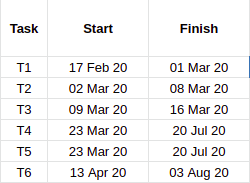
\includegraphics[scale=0.75]{figures/gantt-labels.png}
      \caption{Tasks and deadlines}
      \label{fig:tasks}
    \end{center}
\end{figure}

Furthermore, we built a Gantt Chart \ref{fig:gantt} that illustrates the expected time frame of completion for each task, in weeks. 

\begin{figure}
    \begin{center}
      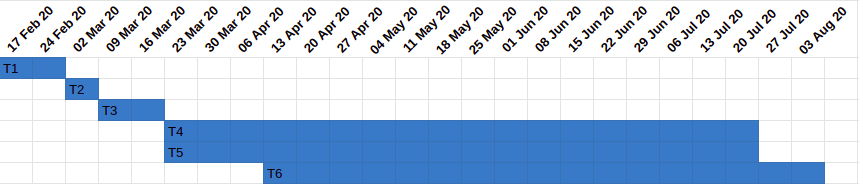
\includegraphics[scale=0.50]{figures/gantt-thesis.png}
      \caption[Thesis research plan]{Gantt Chart of Thesis research plan}
      \label{fig:gantt}
    \end{center}
\end{figure}